\documentclass[12pt, a4paper]{amsart} 

% \usepackage[scaled]{helvet}  % Helvetica font
% \renewcommand*\familydefault{\sfdefault} 
% \usepackage[T1]{fontenc}

\usepackage[T1]{fontenc}
\usepackage{lmodern}
\usepackage{fullpage}   % For narrower margins to save paper when printing
\usepackage{graphicx}   % For graphics
\usepackage{hyperref}   % For hyperreferencs
\hypersetup{colorlinks=False}
\setlength{\hfuzz}{2pt}  % Ignore overlong lines only 2pt over
\renewcommand{\thefootnote}{\fnsymbol{footnote}}  % Use symbolic footnotes
\graphicspath{{pics/}}  % Set path for images
%\setlength{\abovecaptionskip}{4em}  % Space above a figure caption
\pagenumbering{gobble}  % Remove page numbers
\newcommand{\mi}{\text{i}}  % Math i (= sqrt(-1))
\newcommand{\hl}[1]{\textbf{#1}}
%==============================================================================
\begin{document}
\begin{titlepage}

\noindent
\begin{center}
{\fontsize{2cm}{1em}\selectfont CONTOURS}\\[1.5em]
{\LARGE\itshape A Mathematical Coloring Book}\\[4em]
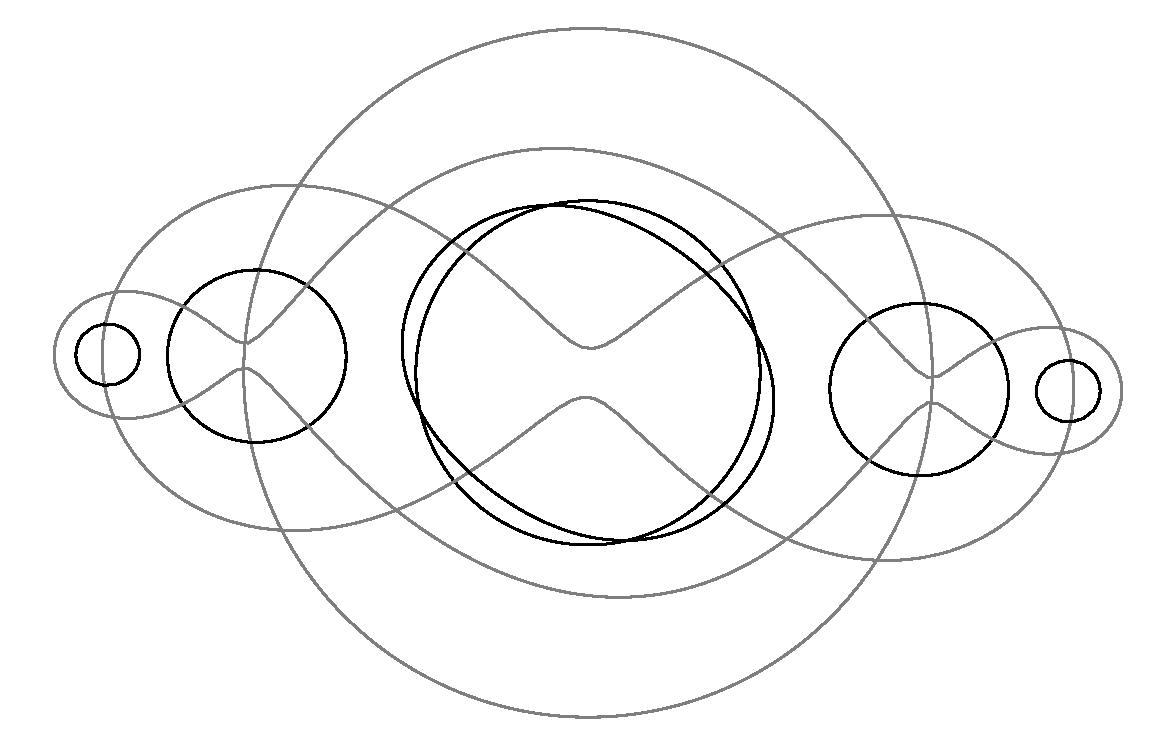
\includegraphics[width=160mm, angle=90]{cover.pdf}\\
\vfill
{\Large ALEXANDER RAICHEV}
\end{center}
\end{titlepage}

%-----------------------------------------------------------------------------
\section*{Introduction}

Q: What is this?

A: This is a mathematical coloring book.
It contains black and white pictures generated by mathematical formulas which you color in for fun.

Q: Why did you make it? 

A: I like math and drawing and decided to combine the two.
Also, I was inspired by \cite{Hamp2009}.

Q: Is this book for kids or adults?

A: Both.
The only requirements are sharp pencils and fine motor skill.

Q: What does the title mean? 

A: Every picture in this book is a contour plot, hence the title `contours'. 
A contour plot of a three-dimensional object is an overlay of several parallel two-dimensional cross sections of the object.
You can think of the object as a landscape and the contour plot as a topographical map of that landscape.

Q: How did you make these pictures?

A: For each picture I chose a function and overlaid sparse contour plots of several of its iterates, an idea I got from \cite{Hamp2009}.
To make the plots, I used Sage~\cite{Sage}, an open-source mathematics software system.

For example, consider the cover picture.
It is a homage to \cite{Hamp2009}, because it involves one of the functions that appears in that book, namely, $f(z) = z^2  - 0.99 + 0.1\mi$.
This function takes as input a complex number $z$, that is, a number of the form $a + b\mi$ where $a, b$ are real numbers and $\mi := \sqrt{-1}$, and then outputs the complex number $z^2 - 0.99 + 0.1\mi$.
For instance, on input $z = 1 + 2\mi$, the output of $f$ is
\begin{align*}
    f(1 + 2\mi) 
    &= 
    (1 + 2\mi)^2 -0.99 +0.1\mi \\
    &= 
    1 + 4\mi +4\mi^2 - 0.99 + 0.1\mi \\
    &= 
    -3.99 + 4.1\mi \quad\text{(since $\mi^2 = -1$)}.
\end{align*}
You can visualize a complex number $a + b\mi$ as a point in the complex plane with horizontal displacement $a$ and vertical displacement $b$; see Figure~\ref{fig:point}.

\begin{figure}[!ht]
\includegraphics[height=70mm]{tutorial_point.pdf}
\caption{
The complex number $1 + 2\mi$ plotted in the complex plane
}
\label{fig:point}
\end{figure}

The graph of $f$ is the set of all points of the form $(z, f(z))$, that is, the set of all pairs of inputs and corresponding outputs of $f$. 
Because both the inputs and outputs of $f$ are complex numbers, they both require two dimensions to draw.
So plotting the graph of $f$ requires four dimensions.
That is too many dimensions.
So I took the absolute value of $f$, which can be plotted in three dimensions and therefore yields a two-dimensional contour plot; see Figure~\ref{fig:3d}.

\begin{figure}[!ht]
(a) 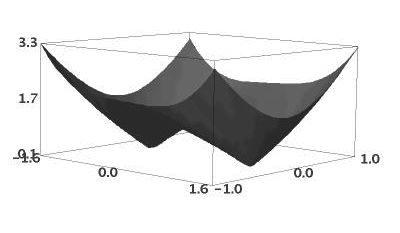
\includegraphics[width=60mm]{tutorial_3d.png}\qquad
(b) 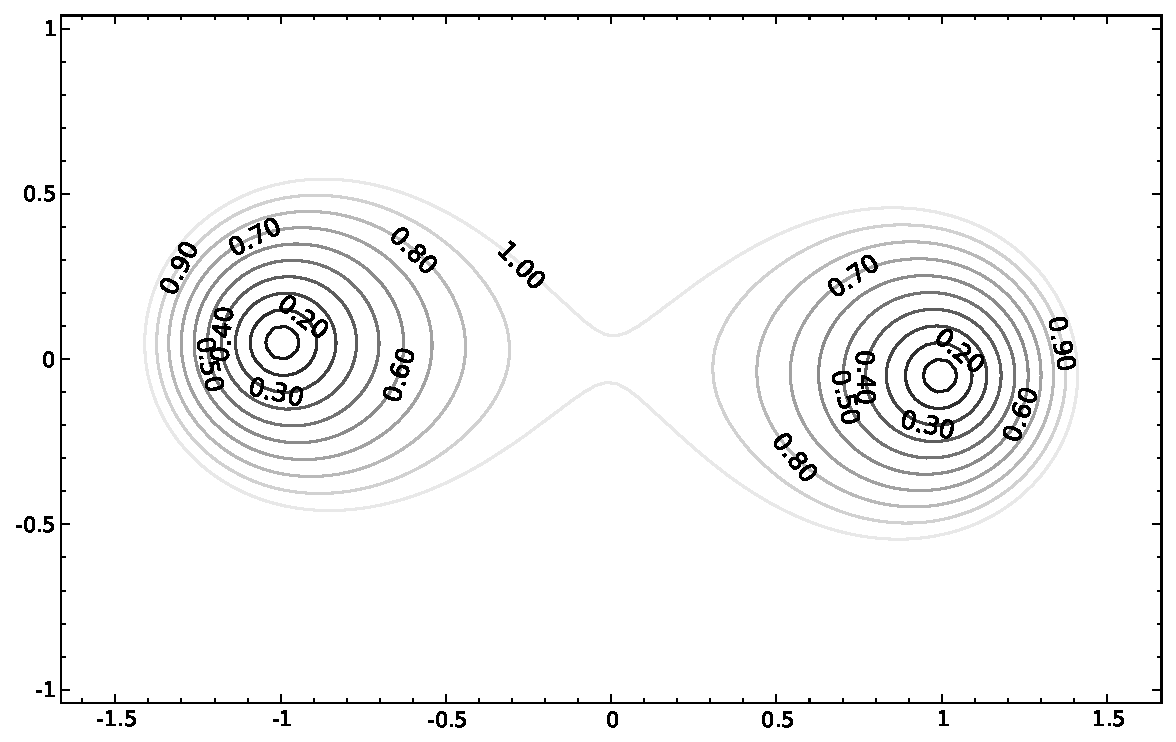
\includegraphics[width=60mm]{tutorial_contour.pdf}
\caption{
(a) Plot of $|f(z)|$ for the complex function $f(z) = z^2  - 0.99 + 0.1\mi$
(b) Contour plot of $|f(z)|$ with contour heights labeled
}
\label{fig:3d}
\end{figure}

The absolute value of a complex number is $|a + b\mi| := \sqrt{a^2 + b^2}$, which is the distance from $a + b\mi$ to the origin in the complex plane and is a nonnegative real number. 
For example, 
\begin{align*}
    |f(1 + 2\mi)| 
    &= 
    |-3.99 + 4.1\mi| \\
    &=
    \sqrt{(-3.99)^2 + (4.1)^2} \\
    &\approx 
    5.72.
\end{align*}
The graph of $|f(z)|$ is the set of all points of the form $(z, |f(z)|)$, which only requires three dimensions to draw, two for the complex number inputs and one for the real number outputs.

Now, to my eye the contour plot in Figure~\ref{fig:3d} is too plain for coloring.
It needs variation.
But how to produce that variation in a systematic way?
Overlay iterates of $f$. 

The $j$th iterate of $f$, written $f^{\circ j}(z)$, is $f$ composed with itself $j$ times.
That is, we feed $z$ to $f$, takes its output and then feed that back into $f$, take its output and then feed that back into $f$, and so on a total of $j$ times.
For example,
\begin{align*}
    f^{\circ 2}(1 + 2\mi)
    &=
    f(f(1 + 2\mi)) \\
    &= 
    f(-3.99 + 4.1\mi) \\
    &= 
    (-3.99 + 4.1\mi)^2 - 0.99 + 0.1\mi \\
    &= 
    -1.8799 - 32.618\mi.
\end{align*}
The zeroth iterate of $f$ is defined to be the identity function $f^{\circ 0}(z) = z$, which simply outputs the input it is given, and the first iterate of $f$ is $f$.
Iterating a function several times, even a simple one, usually produces intricate patterns.
There is even a whole field of mathematics, called `dynamical systems', dedicated to studying the behavior of iterated functions.

Figure~\ref{fig:iterates} shows the contour plots of $|f^{\circ j}(z)|$ for $j = 0, 1, 2$ which comprise the cover page picture.

\begin{figure}[!htb]
(a) 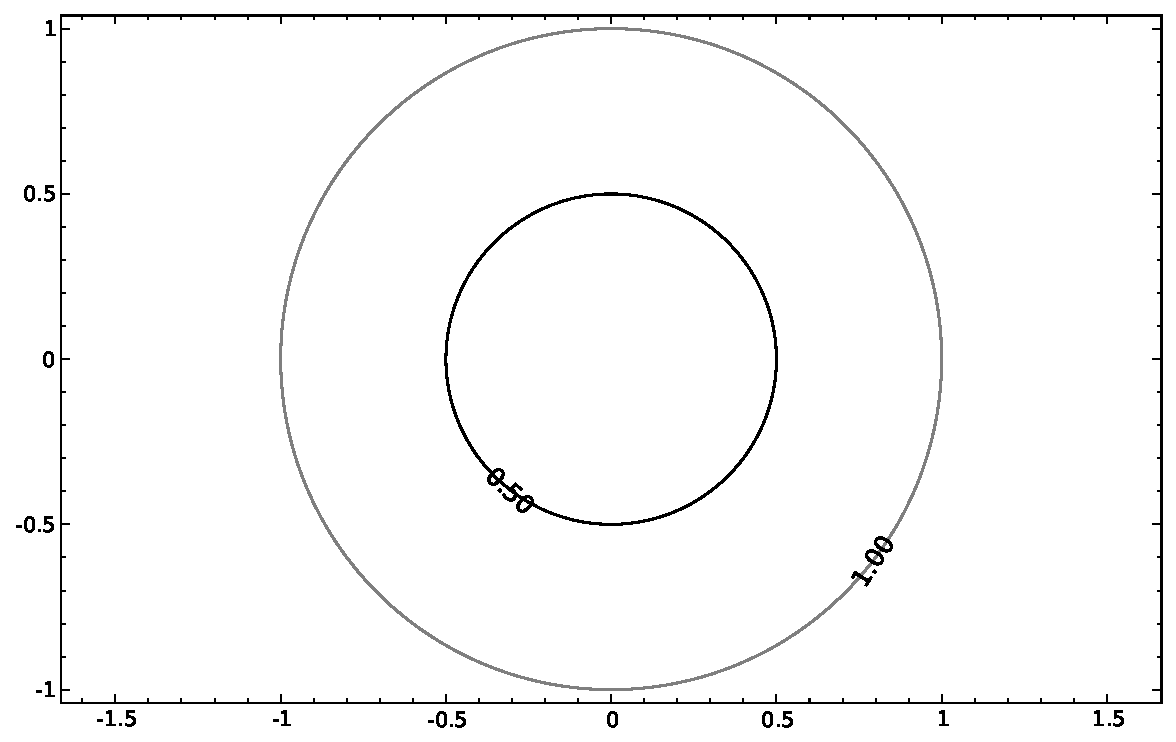
\includegraphics[width=60mm]{tutorial_c0.pdf}\qquad
(b) 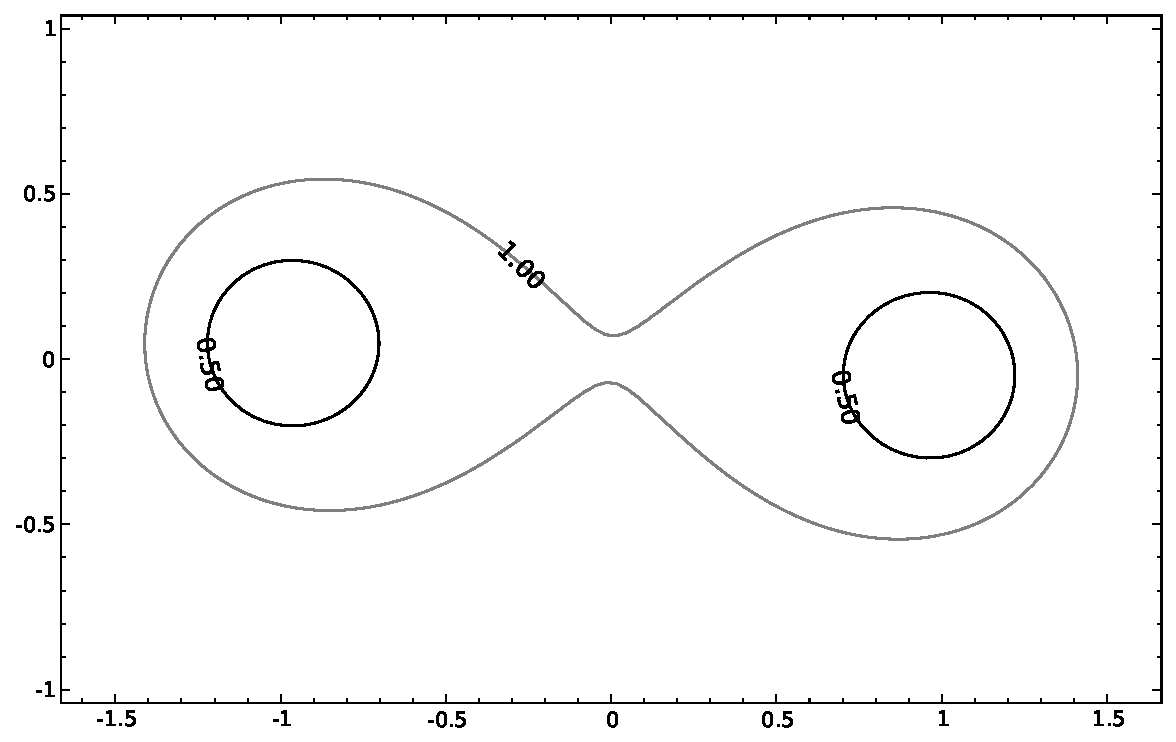
\includegraphics[width=60mm]{tutorial_c1.pdf}\\
(c) 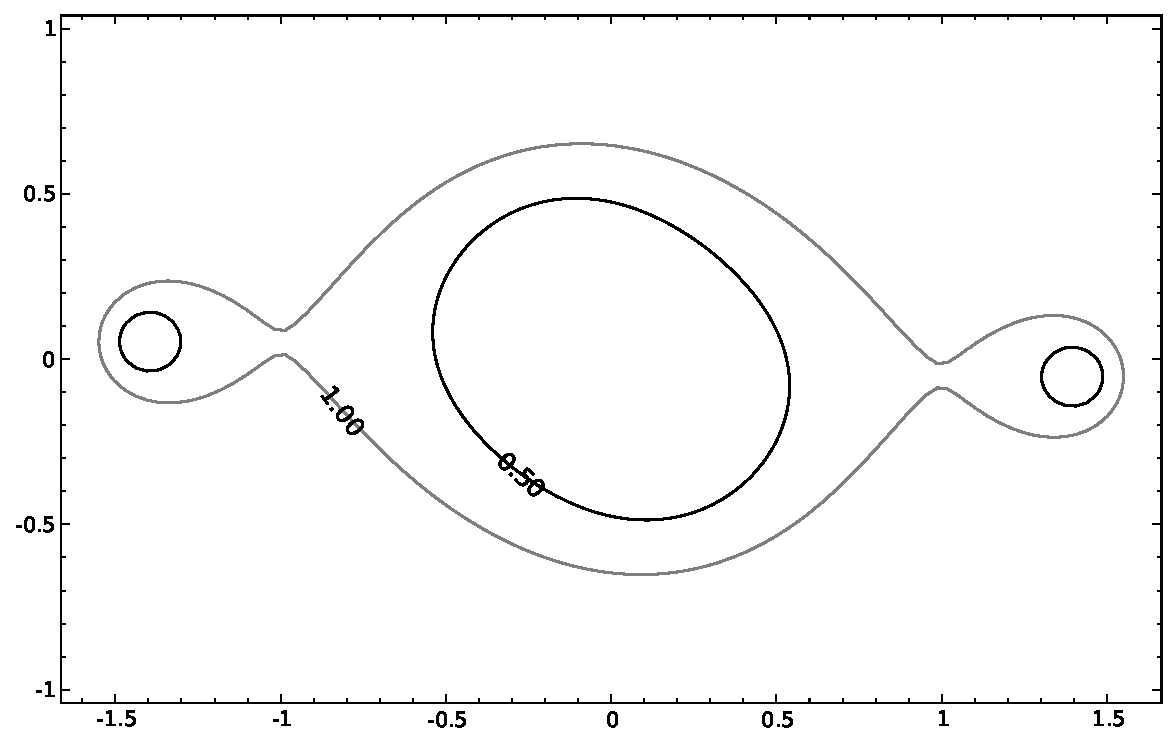
\includegraphics[width=60mm]{tutorial_c2.pdf}\qquad
(d) 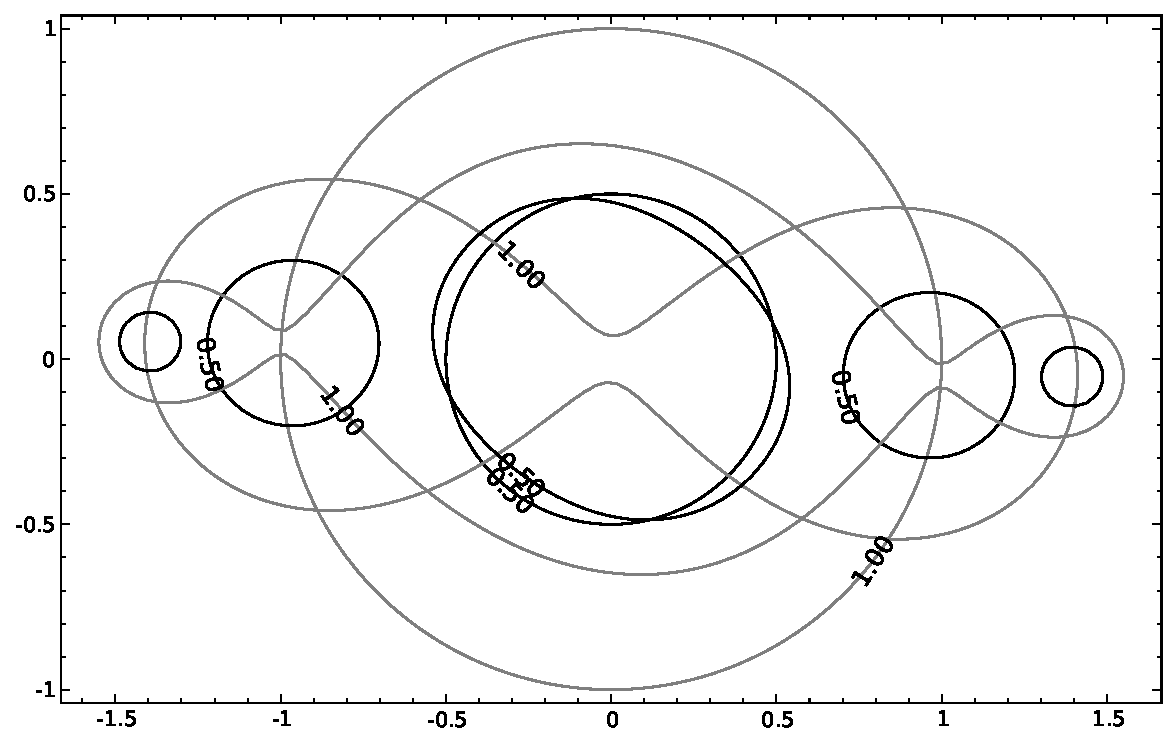
\includegraphics[width=60mm]{tutorial_c012.pdf}
\caption{
Labeled contour plots with contours at heights 0.5 and 1.
(a) $|f^{\circ 0}(z)|$ 
(b) $|f^{\circ 1}(z)|$
(c) $|f^{\circ 2}(z)|$
(d) The overlay of (a), (b), and (c)
}
\label{fig:iterates}
\end{figure}

The final steps in the process are choosing a small collection of contours for each iterate, because too many crowd the picture, and then cropping and rotating the result.
All done by trial and error.

Q: How did you choose the underlying functions?

A: Trial and error again.
I began with linear and quadratic functions and then sprinkled in a few more complicated functions for spice, such as the sine function or the reciprocal of the cubic function.
Finally, I experimented with a couple famous chaotic functions that I found on Wikipedia, namely the Gingerbreadman map and Arnold's cat map.

Q: Can I make pictures like these too?

A: Yes.
One easy way to do so is to run Sage online (for free) and upload this Sage worksheet I made as a template to start drawing:
\url{https://www.dropbox.com/s/yfgagld40te9csf/contours_template.sws}.

%-----------------------------------------------------------------------------
\section*{Acknowledgements}
Thanks to Sasha Rubin for his thoughtful feedback on the introduction and to Poppy Constantine for her...

%-----------------------------------------------------------------------------
\section*{Copyright}

This work was produced by Alexander Raichev March 2013 in Auckland, New Zealand and is licensed under a \href{http://creativecommons.org/licenses/by-sa/3.0/deed.en_US}{Creative Commons Attribution-ShareAlike 3.0 Unported License}.\\[1em]

\includegraphics[width=20mm]{cc_by_sa.png}

%-----------------------------------------------------------------------------
\bibliographystyle{amsalpha}
\bibliography{contours}
\vfill
%-----------------------------------------------------------------------------
\pagebreak
\begin{figure}[!ht]
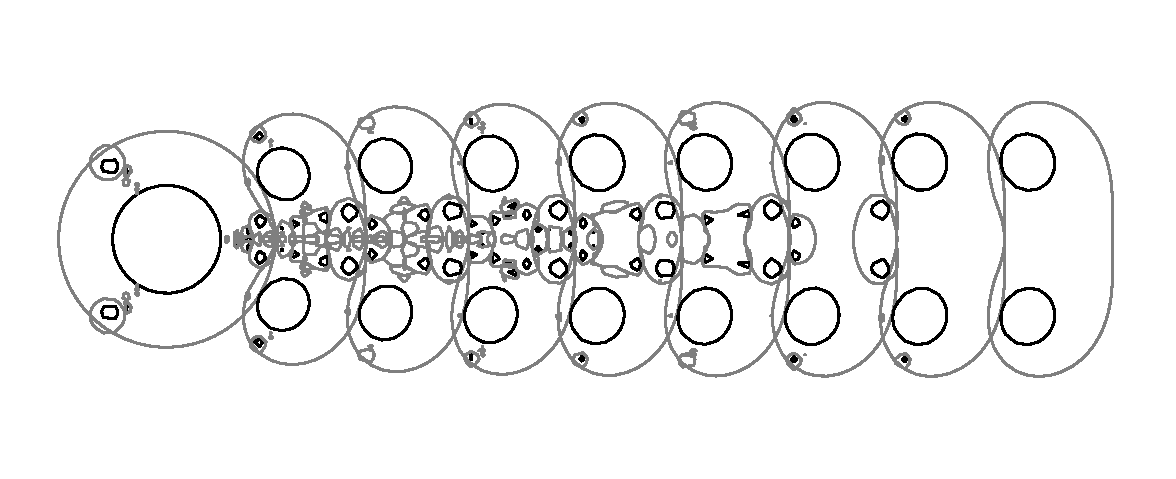
\includegraphics[width=230mm, angle=-90]{caterpillar.pdf}
\caption{
Contours plot of $|f^{\circ j}(z)|$ for $j = 0, 1, \ldots, 8$ and the complex function $f(z) = z - 1 + 1/z^3$.
Contour heights 0.5 and 1.
}
\end{figure}
%-----------------------------------------------------------------------------
\pagebreak
\begin{figure}[!ht]
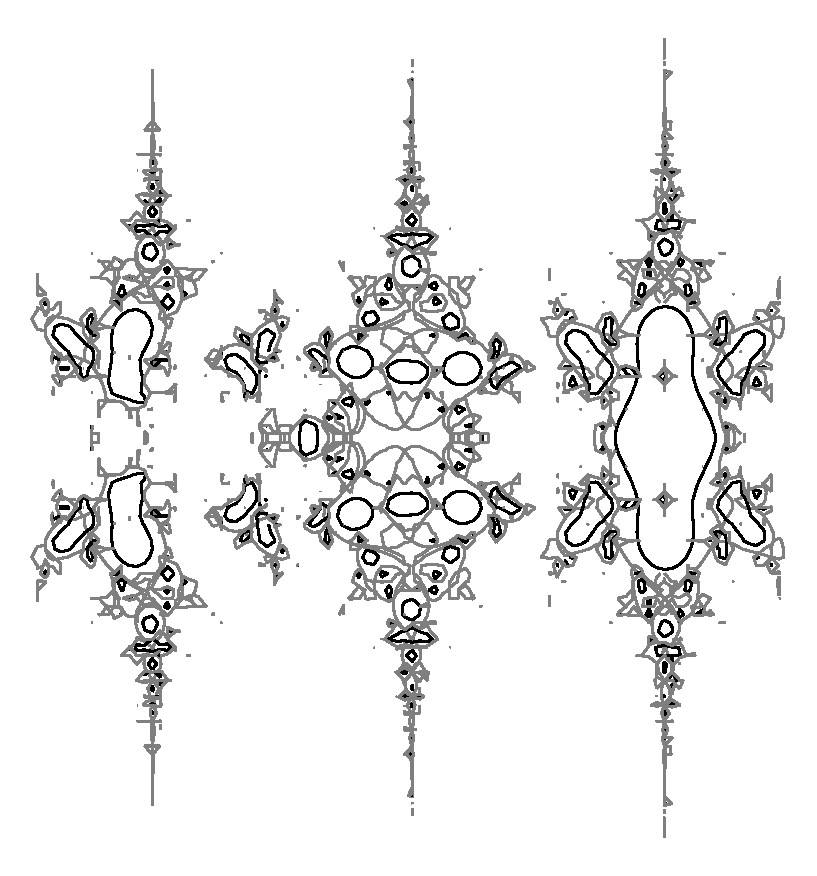
\includegraphics[width=160mm, height=230mm, angle=180]{indian_caterpillar.pdf}
\caption{
Contour plot of $|f^{\circ j}(z)|$ for $j = 2, 3, 4$ and the complex function $f(z) = \sin(z - 1 + 1/z^3)$.
Contour heights 0.5 and 1.
}
\end{figure}
%-----------------------------------------------------------------------------
\pagebreak
\begin{figure}[!ht]
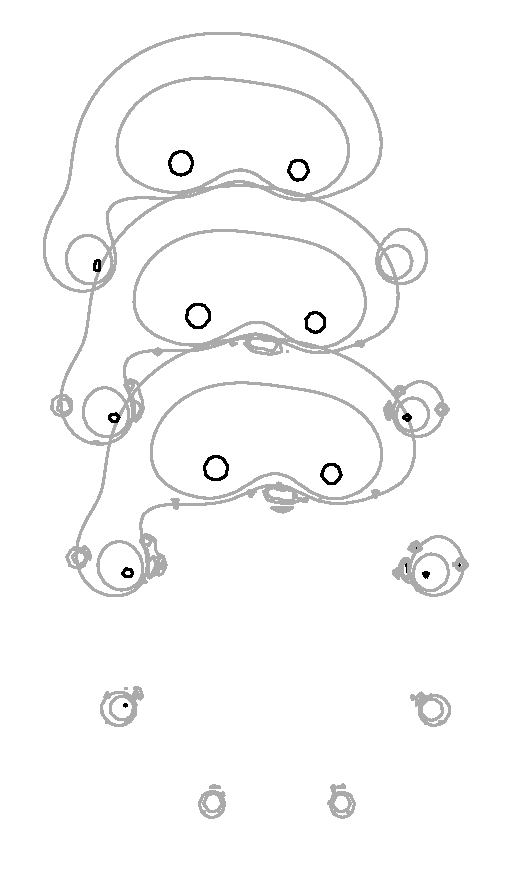
\includegraphics[height=230mm]{three_monkeys.pdf}
\caption{
Contours plot of $|f^{\circ j}(z)|$ for $j = 1, 2, 3$ and the complex function $f(z) = z + 1 -0.9\mi + 1/z^7$.
Contour heights 0.2, 0.75, and 1.
}
\end{figure}
%-----------------------------------------------------------------------------
\pagebreak
\begin{figure}[!ht]
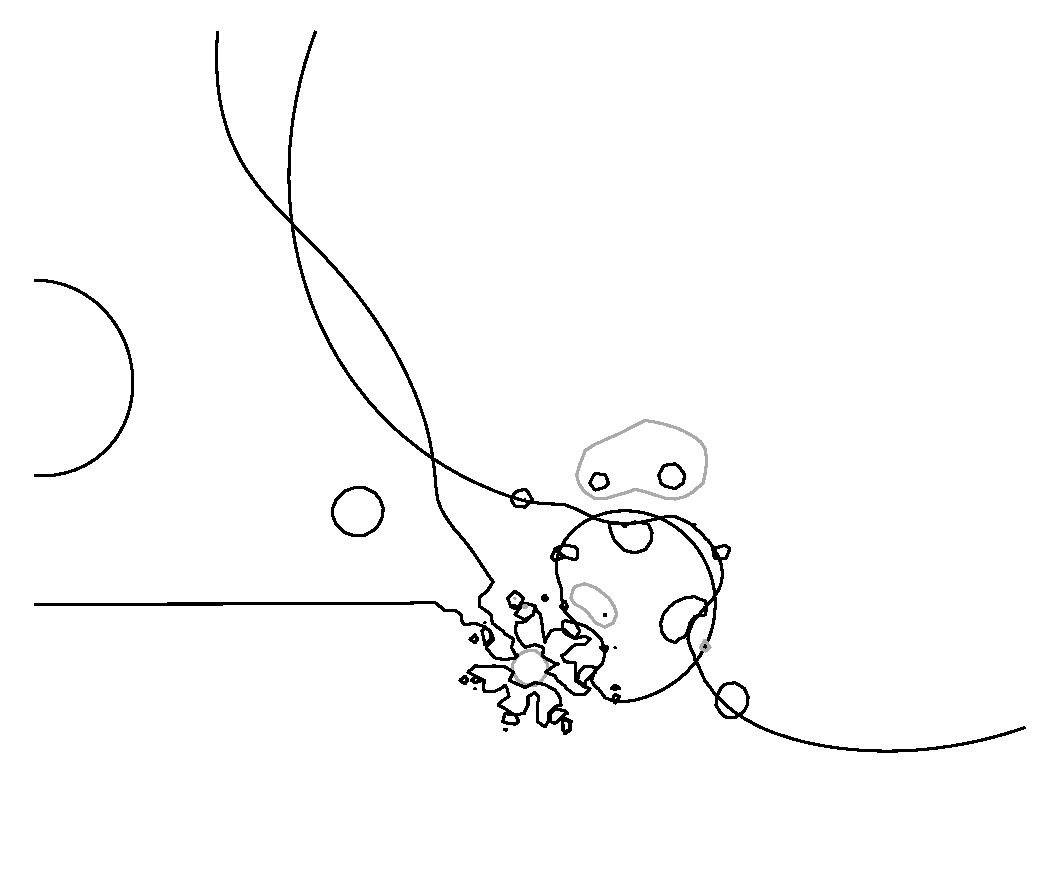
\includegraphics[width=160mm, height=170mm]{three_monkeys_eaten.pdf}
\caption{
Contours plot of $|f^{\circ j}(z)|$ for $j = 1, 2, 3$ and the complex function $f(z) = \log(z + 1 -0.9\mi + 1/z^7)$.
Contour heights 0.1, 1, and 10.
}
\end{figure}
%-----------------------------------------------------------------------------
\pagebreak
\begin{figure}[!ht] 
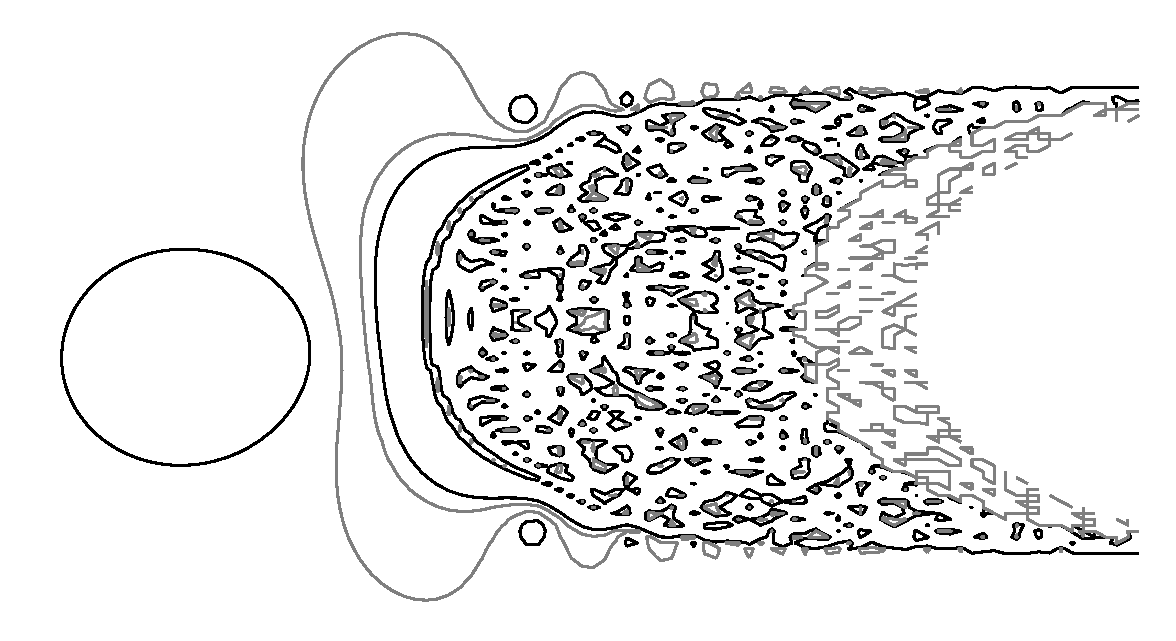
\includegraphics[width=230mm, angle=-90]{mr_fancy_pants.pdf}
\caption{
Contour plot of $\sin(|f^{\circ 2}(z)|)$ for the complex function $f(z) = \exp(z) - 0.99 + 0.1\mi$.
Contour heights 0.5 and 0.9.
}
\end{figure}
%-----------------------------------------------------------------------------
\pagebreak
\begin{figure}[!ht]
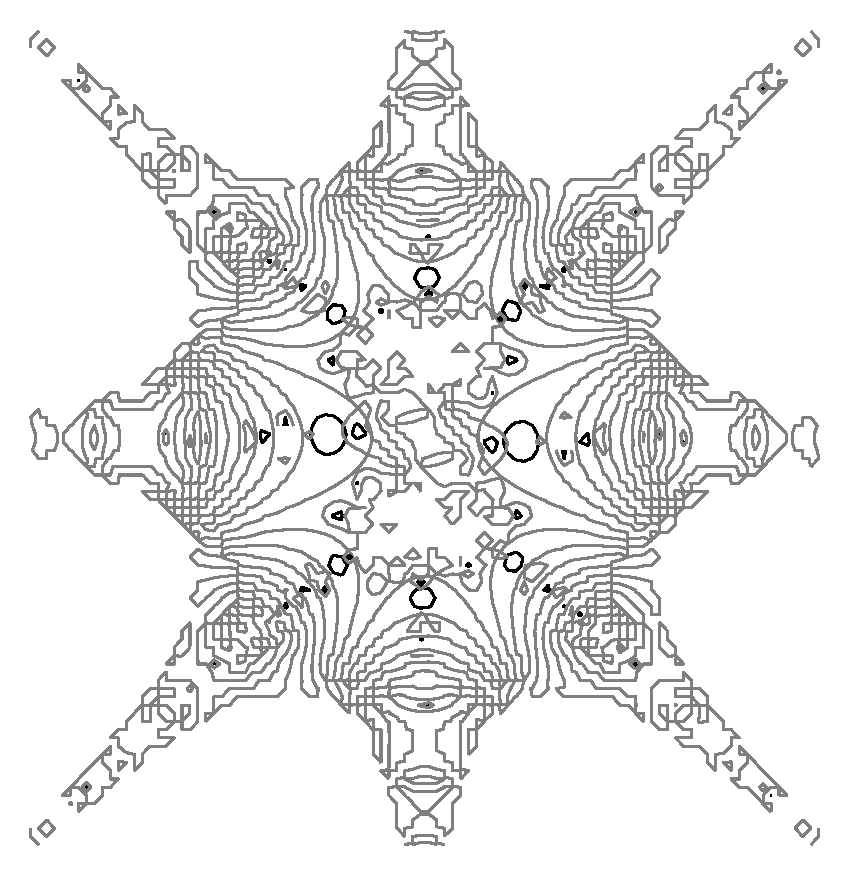
\includegraphics[width=160mm]{mite.pdf}
\caption{
Contour plot of $|f^{\circ j}(z)|$ for $j = 1, 2$ and the complex function $f(z) = \tan(z^2  + z^2 - 0.99 + 0.1\mi)$.
Contour heights 0.5 and 1.
}
\end{figure}
%-----------------------------------------------------------------------------
\pagebreak
\begin{figure}[!ht] 
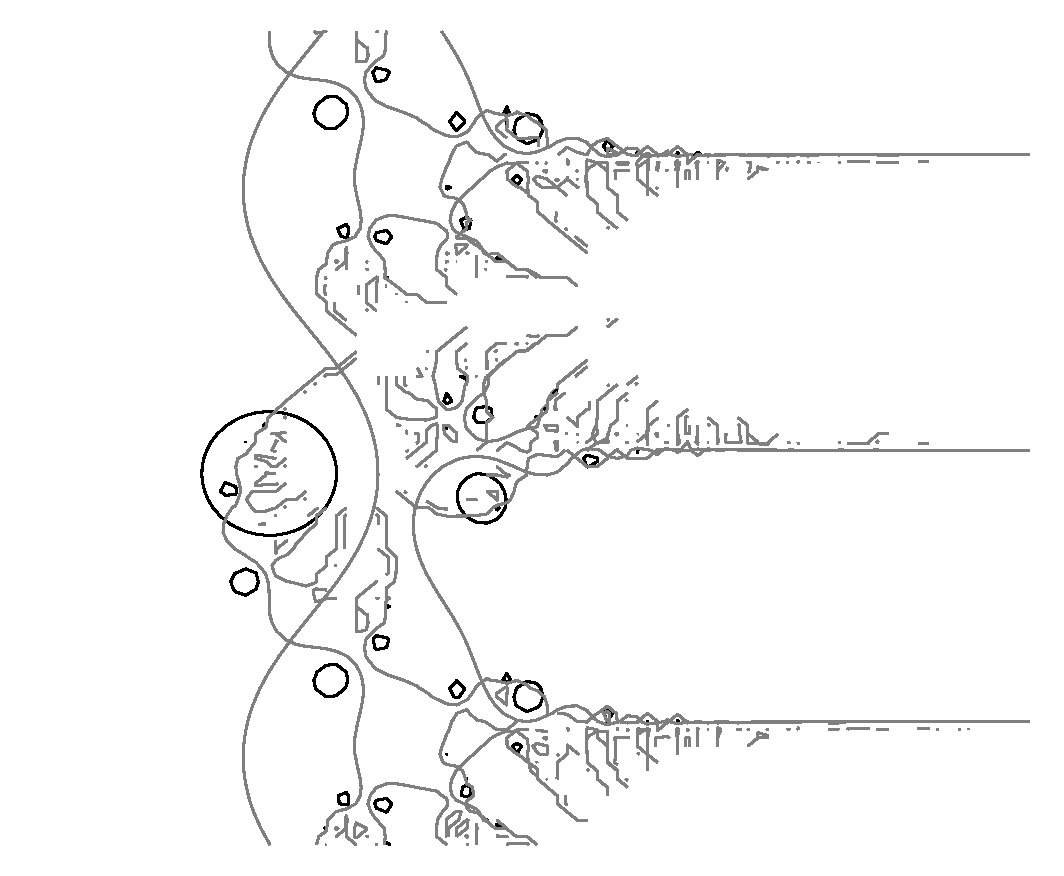
\includegraphics[height=160mm, angle=-90]{landscape.pdf}
\caption{
Contour plot of $|f^{\circ j}(z)|$ for $j=1, 2, \ldots, 7$ and the complex function $f(z) = \exp(z) + 0.1 + 0.3\mi$.
Contour heights 0.2 and 0.5.
}
\end{figure}
%-----------------------------------------------------------------------------
\pagebreak
\begin{figure}[!ht] 
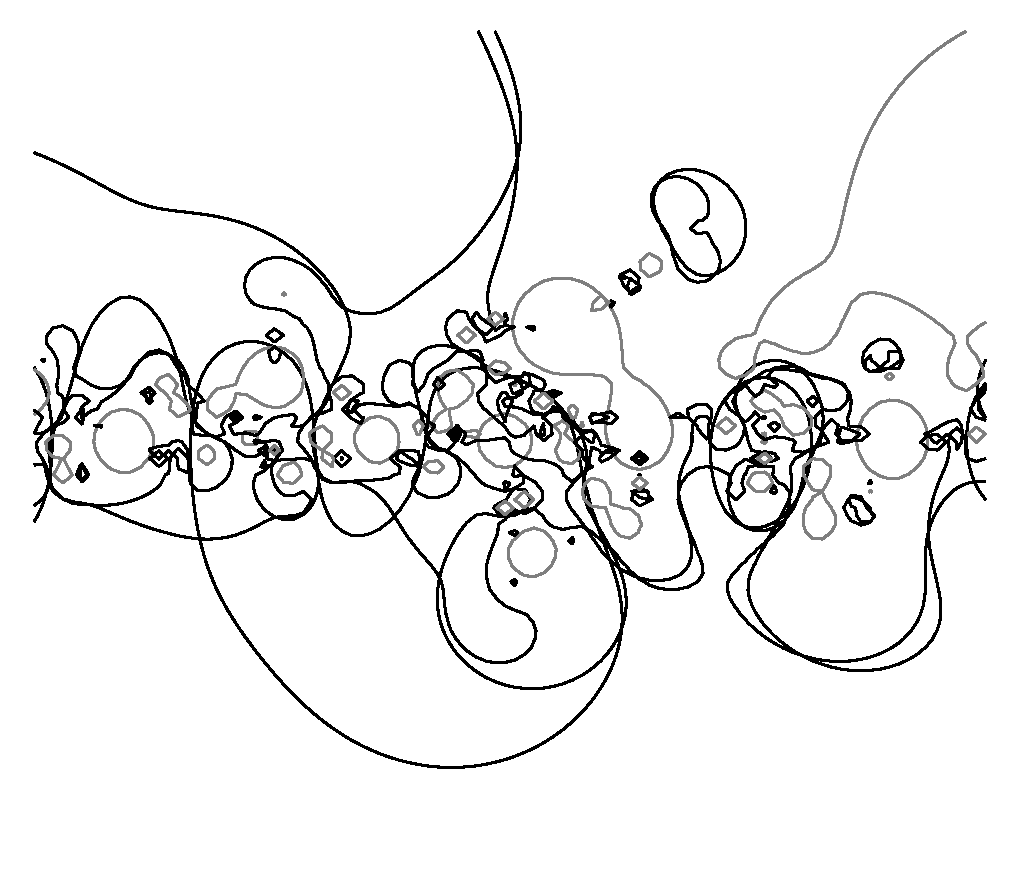
\includegraphics[height=160mm, angle=90]{embryos.pdf}
\caption{
Contour plot of $|f^{\circ j}(z)|$ for $j=1, 2, 3, 4$ and the complex function $f(z) = \cot(z)(1/z - 0.3 + 0.7\mi)$.
Contour heights 1 and 10.
}
\end{figure}
%-----------------------------------------------------------------------------
\pagebreak
\begin{figure}[!ht] 
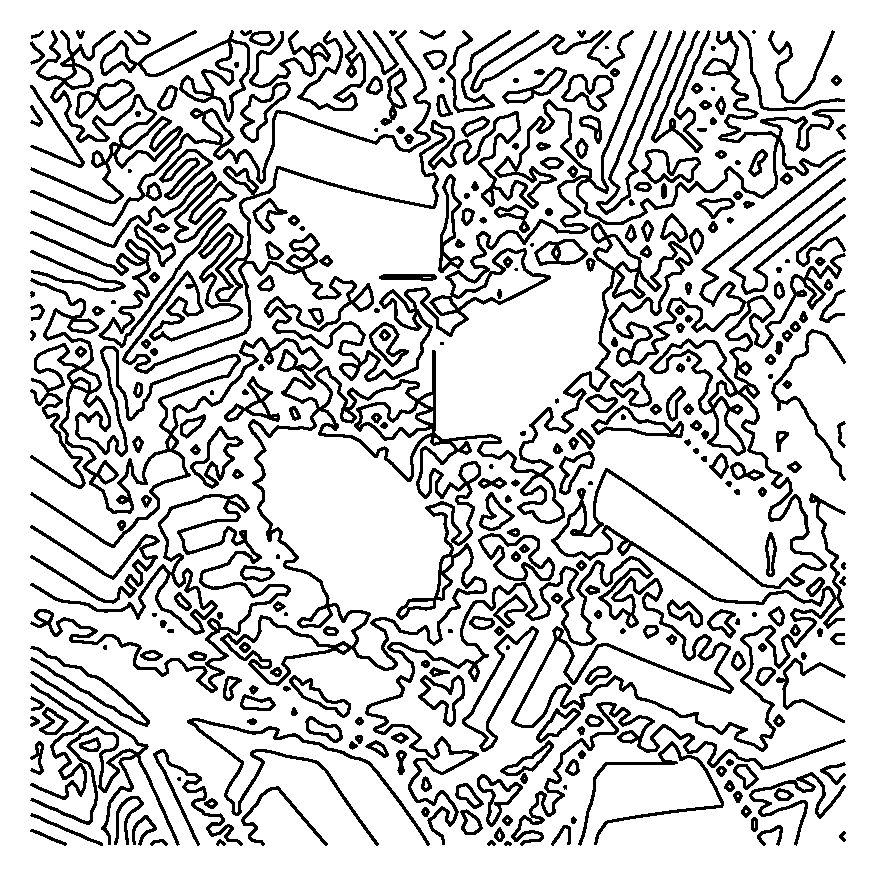
\includegraphics[width=160mm, height=210mm]{gingerbreadman.pdf}
\caption{
Contour plot of $\sin(x_{65} y_{65})$ for $(x_{65}, y_{65}) = f^{\circ 65}(x, y)$ and the Gingerbreadman map $f(x, y) = (1 - y + |x|, x)$.
Contour height 0.
}
\end{figure}
%-----------------------------------------------------------------------------
\pagebreak
\begin{figure}[!ht] 
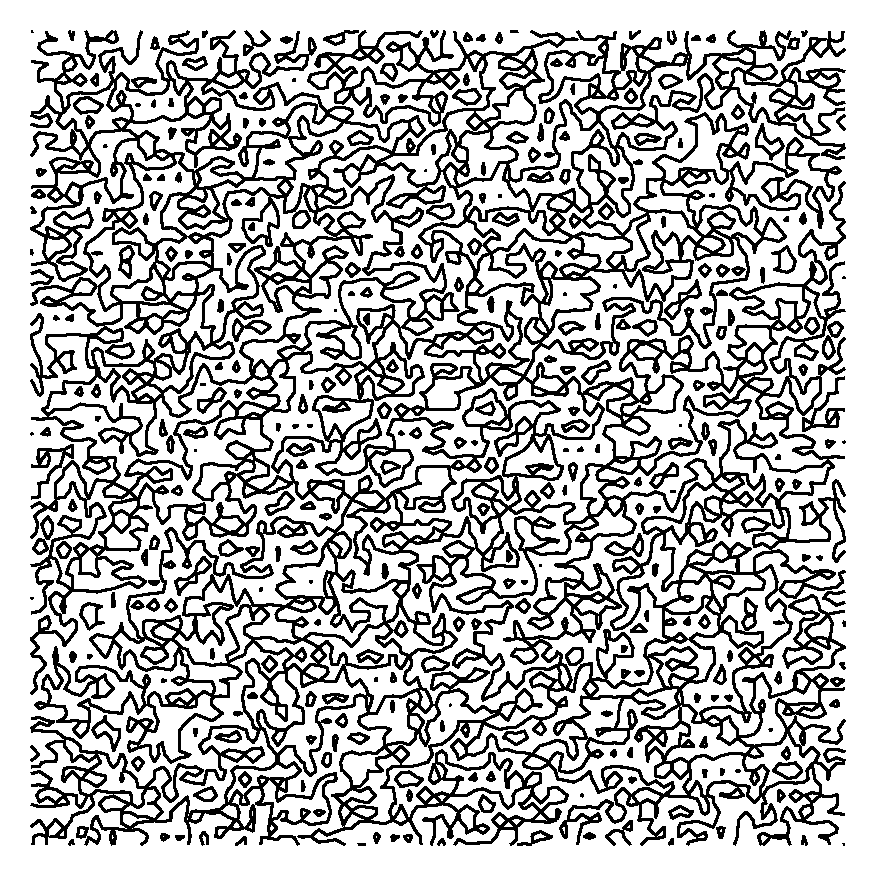
\includegraphics[width=160mm, height=210mm]{arnolds_cat3.pdf}
\caption{
Contour plot of $\tan(x_8 + y_8)$ for $(x_8, y_8) = f^{\circ 8}(x, y)$ and  $f(x, y) = (2x + y, x + y) \mod 3$.
Contour height 0.
}
\end{figure}
%-----------------------------------------------------------------------------
% \pagebreak
% \begin{figure}[!ht] 
% \includegraphics[height=130mm, angle=-90]{orchid.pdf}
% \caption{
% Contour plot of the complex function $\sin(\Re(\Gamma(z)/z)))$.
% }
% \end{figure}

%-----------------------------------------------------------------------------
% \pagebreak
% \begin{figure}[!ht] 
% \includegraphics[width=160mm, height=210mm]{duffing.pdf}
% \caption{
% Contour plot of $\sin(x_{11} y_{11})$ for $(x_{11}, y_{11}) = f^{\circ 11}(x, y)$ and Duffing's map $f(x, y) = (y, -0.2x + 2.75y - y^3) \mod 1$.
% }
% \end{figure}

%-----------------------------------------------------------------------------
% \pagebreak
% \begin{figure}[!ht] 
% \includegraphics[width=160mm, height=210mm]{tinkerbell.pdf}
% \caption{
% Contour plot of $\sin(x_2 + y_2))$ for $(x_2, y_2) = f^{\circ 2}(x, y)$ and the Tinkerbell map $f(x, y) = (x^2 - y^2 + 0.3x + 0.6y, 2*x*y + 2x + 0.27y)$.
% }
% \end{figure}
\end{document}
